\documentclass[aspectratio=169,usepdftitle=true,t]{beamer}

\usepackage[T1]{fontenc}
\usepackage[utf8]{inputenc}
\usepackage{microtype}
\usepackage[main=english]{babel}
\usepackage{siunitx}
%\usetheme[noemblem,theorems]{colorful-dream}
\usepackage{bm}
\usepackage[absolute,overlay]{textpos}
\usepackage{subcaption}
%\usepackage{transparent}
\newcommand{\rmn}[1]{\mathrm{#1}}

\usepackage{xcolor}
\newcommand{\gray}[1]{\textcolor{gray}{#1}}

\usepackage{tikz}
%\usepackage{multimedia}
%\usepackage{movie15}
\usepackage{animate}

\definecolor{color1}{HTML}{2d5d7b}
\definecolor{color2}{HTML}{8a0a24}
\definecolor{color3}{HTML}{d99808}
\definecolor{color4}{HTML}{9fdab8}



\newcommand{\ud}{\,\mathrm{d}}
\newcommand{\bnabla}{\bm{\nabla}}
\newcommand{\bcdot}{\bm{\cdot}}
\newcommand{\red}[1]{\textcolor{red}{#1}}
\newcommand{\green}[1]{\textcolor{green}{#1}}
%\newcommand{\gray}[1]{\textcolor{gray}{#1}}
%\newcommand{\rmn}[1]{\mathrm{#1}}
\newcommand{\ccp}[1]{\textcolor{red}{\textbf{[CP: #1]}}}
\newcommand{\cp}[1]{\textcolor{red}{#1}}
\newcommand{\TB}[1]{\textcolor{orange}{\textbf{[TB: #1]}}}
\newcommand{\lmp}[1]{\textcolor{blue}{\textbf{[LMP: #1]}}}
\newcommand{\lp}[1]{\textcolor{blue}{#1}}

%\tikzset{
%	invisible/.style={opacity=0},
%	visible on/.style={alt={#1{}{invisible}}},
%	alt/.code args={<#1>#2#3}{%
%		\alt<#1>{\pgfkeysalso{#2}}{\pgfkeysalso{#3}} % \pgfkeysalso doesn't change the path
%	},
%}

%\tikzset{
%	%Define standard arrow tip
%	%	>=stealth',
%	%Define style for boxes
%	punkt/.style={
%		rectangle,
%		rounded corners,
%		draw=black, very thick,
%		text width=6.5em,
%		minimum height=2em,
%		text centered},
%	% Define arrow style
%	pil/.style={
%		->,
%		thick,
%		shorten <=2pt,
%		shorten >=2pt,}
%}
%
%\tikzstyle{na} = [baseline=-.5ex]
%\everymath{\displaystyle}
%\tikzstyle{every picture}+=[remember picture]

\graphicspath{./Figures/}

\title{Notes on volume integrals and Fourier decomposition}
\subtitle{}
%\institute{Leibniz-Institute for Astrophysics \(\circ\) Potsdam}

%\date{Nils Bohr Institute \(\circ\) Copenhagen, 17 June 2025}

%\author{\textbf{Lorenzo Maria Perrone}, Thomas Berlok, Ewald Puchwein, Christoph Pfrommer}
%\email{lperrone@aip.de}

%\outro{Ann Arbor, 28 June 2024}

%\SetEmblem[university Ulm]{Example Institute}{\faCode}

% tikz code is possible as well!
% TODO: you may want to change this if you do not have downloaded the image
%\begin{tikzpicture}
%	\node[anchor=south west,inner sep=0] (image) at (0,0) {\includegraphics[width=1.0\linewidth]{Figures/magnetic_fields_buoyancy.pdf}};
%\end{tikzpicture}
%\titleimage{\includegraphics[width=1.0\linewidth]{Figures/first_slide.pdf}}

% just an example command
\newcommand\twosplit[3][t]{%
	\begin{columns}[#1]
		\begin{column}{0.475\linewidth}
			#2
		\end{column}\hfill
		\begin{column}{0.475\linewidth}
			#3
		\end{column}
	\end{columns}
}

%\usepackage[backend=bibtex8,style=authoryear-comp, citestyle=authoryear-comp, sorting=nty,natbib=true]{biblatex}
\usepackage[backend=bibtex8,natbib=true]{biblatex}
%\addbibresource{MyLibrary2.bib}
\begin{document}
	
\maketitle


\begin{frame}
	\begin{itemize}
		\item assume periodic domain $V$
		\item expand magnetic field in Fourier series
		\begin{align*}
			\bm B (\bm x) = \sum_{\bm k}  \hat{ \bm B}_{\bm k} e^{i \bm k \bcdot \bm x }, \label{eq:synthetic_magnetic_field}
		\end{align*}
		\item compute energy density 
		\begin{align*}
			e_B (\bm x) = \frac{\bm B^2}{8\pi},
		\end{align*}
		\item explicitly:
		\begin{align*}
			&8 \pi e_B (\bm x) = \sum_{\bm k}  |\hat{ \bm B}({\bm k})|^2 + \sum_{\bm k \neq \bm k'} \Re \left\lbrace \hat{ \bm B}^* ({\bm k}) \bcdot \hat{ \bm B} ({\bm k'}) e^{i (\bm k' - \bm k) \bcdot\bm x } \right\rbrace 
		\end{align*}
	\end{itemize}
	
\end{frame}

\begin{frame}{Integrate over entire volume $V$}
	\begin{itemize}
		\item Report below energy density:
		\begin{align*}
			&8 \pi e_B (\bm x) = \sum_{\bm k}  |\hat{ \bm B}({\bm k})|^2 + \sum_{\bm k \neq \bm k'} \Re \left\lbrace \hat{ \bm B}^* ({\bm k}) \bcdot \hat{ \bm B} ({\bm k'}) e^{i (\bm k' - \bm k) \bcdot\bm x } \right\rbrace 
		\end{align*}
		\item compute \textbf{total} energy $E_{B,\mathrm{tot}} = \int_V e_B \ud^3 \bm x$:
		\begin{align*}
			E_{B,\mathrm{tot}} = \sum_{\bm k}  \frac{|\hat{ \bm B}({\bm k})|^2}{8 \pi} V
		\end{align*}
		
	\end{itemize}
\end{frame}

\begin{frame}{What if we integrate over only subvolume $V' < V$?}
	\begin{itemize}
		\item Total energy of the subvolume $V' = L'_x L'_y L'_z$ centered around $\bm x_0$:
		%		$E_B (V') = \int_{V'} e_B \ud^3 \bm x$:
		\begin{align*}
			&E_B(V') = \frac{E_{B,\mathrm{tot}}}{V}  V' \nonumber \\
			&+ \sum_{\bm k \neq \bm k'} \Re \left\lbrace \frac{\hat{ \bm B}^* ({\bm k}) \bcdot \hat{ \bm B} ({\bm k'})}{8\pi}  \right\rbrace \cos((\bm k - \bm k') \bcdot\bm x_0) \prod_{i=x,y,z} \mathrm{sinc} \left( \frac{(\bm k - \bm k')_i L'_i}{2} \right)  V'
		\end{align*}
	\end{itemize}
\end{frame}

\begin{frame}{Example 1: statistically homogeneous field}
	\begin{textblock}{9}(0.5,2)
		\begin{itemize}
			\item Total energy of the subvolume $V' = L'_x L'_y L'_z$ centered around $\bm x_0$:
			%		$E_B (V') = \int_{V'} e_B \ud^3 \bm x$:
			\begin{align*}
				&E_B(V', \bm x_0) = \frac{E_{B,\mathrm{tot}}}{V}  V' + \nonumber \\
				&+ \sum_{\bm k \neq \bm k'} \left[ \Re \left\lbrace \frac{\hat{ \bm B}^* ({\bm k}) \bcdot \hat{ \bm B} ({\bm k'})}{8\pi}  \right\rbrace \cos((\bm k - \bm k') \bcdot\bm x_0) \times \right. \\
				& \left. \times \prod_{i=x,y,z} \mathrm{sinc} \left( \frac{(\bm k - \bm k')_i L'_i}{2} \right) \right] V'
			\end{align*}
		\end{itemize}
	\end{textblock}
	\begin{textblock}{15}(0.5,12)
		\begin{itemize}
			\item $E_B(V', \bm x_0)$ roughly independent of $\bm x_0$: first term dominates
		\end{itemize}
	\end{textblock}
	\begin{textblock}{6}(10,1)
		\begin{figure}
			\centering
			\includegraphics[width=1.0\columnwidth]{Figures/2a.magnetic_energy_fixed_filter_regions.pdf}
		\end{figure}
	\end{textblock}
\end{frame}

\begin{frame}{Example 2: inhomogeneous field}
	\begin{textblock}{9}(0.5,2)
		\begin{itemize}
			\item Total energy of the subvolume $V' = L'_x L'_y L'_z$ centered around $\bm x_0$:
			%		$E_B (V') = \int_{V'} e_B \ud^3 \bm x$:
			\begin{align*}
				&E_B(V', \bm x_0) = \frac{E_{B,\mathrm{tot}}}{V}  V' + \nonumber \\
				&+ \sum_{\bm k \neq \bm k'} \left[ \Re \left\lbrace \frac{\hat{ \bm B}^* ({\bm k}) \bcdot \hat{ \bm B} ({\bm k'})}{8\pi}  \right\rbrace \cos((\bm k - \bm k') \bcdot\bm x_0) \times \right. \\
				& \left. \times \prod_{i=x,y,z} \mathrm{sinc} \left( \frac{(\bm k - \bm k')_i L'_i}{2} \right) \right] V'
			\end{align*}
		\end{itemize}
	\end{textblock}
	\begin{textblock}{15}(0.5,12)
		\begin{enumerate}
			\item empty $V'$:  $E_B(V', \bm x_0) \approx 0$, first term and second term comparable (cancellation)
			\item ``dense'' $V'$: $E_B(V', \bm x_0)$ comparable to \textbf{total} $E_B$ of total $V$, second term can dominate!
		\end{enumerate}
	\end{textblock}
	\begin{textblock}{6}(10,1)
		\begin{figure}
			\centering
			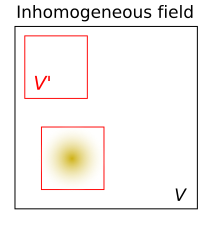
\includegraphics[width=0.9\columnwidth]{Figures/inhomogeneous_field.pdf}
		\end{figure}
	\end{textblock}
\end{frame}

\begin{frame}{Conclusions}
	\begin{itemize}
		\item Both terms are important when computing energies and energy densities (especially when field non statistically homogeneous)
		\item same reasoning applies to filtered energies
		\item filtered energy densities have a physical meaning
	\end{itemize}
\end{frame}

%\begin{textblock}{15}(0.5,1)
%	\begin{figure}
%		\centering
%		\includegraphics[width=1.0\columnwidth]{Figures/kinetic_magnetic_amplitudes.pdf}
%	\end{figure}
%\end{textblock}
%
%\begin{frame}[c]{Outline}
%    
%\end{frame}



\end{document}